\documentclass[ngerman,compress]{beamer}

\mode<presentation>
{
  \useoutertheme[footline=titleinstituteauthor]{c4}
  \useinnertheme{circles}
  \usecolortheme{c4}
  %\setbeamercovered{transparent}
  \setbeamercovered{highly dynamic}
}

\usepackage{babel}
\usepackage[utf8]{luainputenc}
\usepackage{fontspec}
\usepackage{listings}
\usepackage{color}
\usepackage{siunitx}
\usepackage{tikz}
\usetikzlibrary{calc,arrows}

% Multimedia
%\usepackage{multimedia}

\definecolor{dark-green}{RGB}{5, 148, 5}
\lstset{
language=C,
basicstyle=\ttfamily\small,
keywordstyle=\color{blue}\bfseries,
commentstyle=\color{dark-green}\slshape,
stringstyle=\color{purple},
breaklines=true,
breakatwhitespace=true,
prebreak=\raisebox{0ex}[0ex][0ex]{\ensuremath{\hookleftarrow}},
tabsize=2,
numbers=left,
numberstyle=\tiny,
moredelim=[is][\sl]{$}{$},
escapechar=\%,
morekeywords={size_t, _Bool, uint8_t, int8_t, uint16_t, int16_t, uint32_t, int32_t}
}

\title[Audio - u23 2013]
{\textbf{Audio}\\u23 2013}

\author[florob <florob@babelmonkeys.de>]
{andy, florob, gordin, ike, meise, tobix, zakx}

\institute[Chaos Computer Club Cologne]
{
Chaos Computer Club Cologne e.V.\\
http://koeln.ccc.de \\
}

\date{2013-11-18}

\pgfdeclareimage[height=1cm]{barcode}{./c4-logo}
\logo{\pgfuseimage{barcode}}


% Folgendes sollte gelC6scht werden, wenn man nicht am Anfang jedes
% Unterabschnitts die Gliederung nochmal sehen möchte.
%\AtBeginSection[]
%{
%  \begin{frame}<beamer>
%    \frametitle{Gliederung}
%    \tableofcontents[currentsection,currentsubsection]
%  \end{frame}
%}

% Falls Aufzählungen immer schrittweise gezeigt werden sollen, kann
% folgendes Kommando benutzt werden:
%\beamerdefaultoverlayspecification{<+->}


\begin{document}

\begin{frame}
  \titlepage
\end{frame}

\begin{frame}{A/D-Wandlung}
	\begin{itemize}
		\item Periodisches einlesen von Werten (\emph{Abtastung})
		\item Sampling-Frequenz $f_s$, z.\,B.\ \SI{44100}{\kilo\hertz}
		\item Signale bis $f_g = f_s/2$, sonst Aliasing
		\item Tiefpass zum beschränken der Eingangsfrequenzen
		\item Diskretisieren der Abtastwerte (\emph{Sample})
		\item $2^b-1$ Stufen
		\item z.\,B.\ 16-bit $\Rightarrow$ 65535 Abtastniveaus
	\end{itemize}
\end{frame}

\begin{frame}{Aliasing}
	\begin{columns}
		\column{0.6\linewidth}
		\begin{block}{Nyquist-Shannon-Theorem}
			$f_s > 2\cdot f_g$, für perfekte Rekonstruktion
		\end{block}
		\column{0.4\linewidth}
		\begin{itemize}
			\item $f_\mathrm{rot} = \SI{3}{\hertz}$
			\item<2-> $f_s=\SI{4}{\hertz}$
			\item<3-> $f_\mathrm{blau} = \SI{1}{\hertz}$
		\end{itemize}
	\end{columns}
	\begin{figure}[h]
		\begin{center}
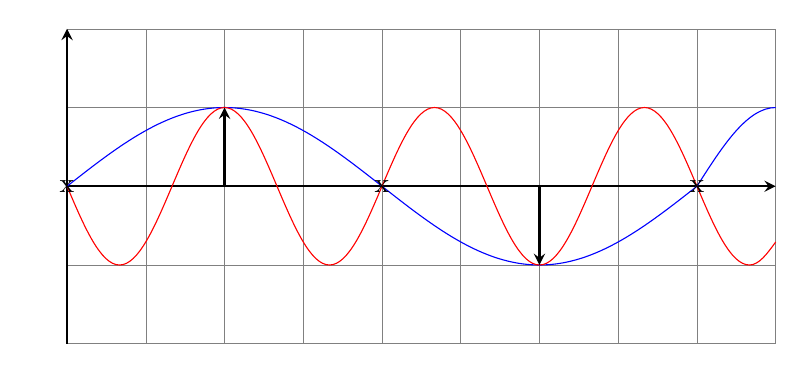
\begin{tikzpicture}[,>=stealth]
	\path[] (-0.5,-2) -- (9,-2) -- (9,2) -- (-0.5,2);
	\draw[help lines] (0,-2) grid (9,2);
	\draw[thick,->] (0,0) -- (9,0);
	\draw[thick,->] (0,-2) -- (0,2);
	\draw<3-> [blue] (0,0) sin (2,1) cos (4,0) sin (6,-1) cos (8,0) sin (9,1);
	\draw[red] (0,0) sin (2/3,-1) cos (4/3,0) sin (2,1)
		cos (8/3,0) sin (10/3, -1) cos (4,0)
		sin (14/3,1) cos (16/3,0) sin (18/3,-1)
		cos (20/3,0) sin (22/3,1) cos (8,0)
		sin (26/3,-1) cos ($(9,0) + sin(-135)*(0,1)$);

	\draw<2-> [thick] (0,0) node {x};
	\draw<2-> [thick,->] (2,0) -- ($(2,0) + sin(90)*(0,1)$);
	\draw<2-> [thick] (4,0) node {x};
	\draw<2-> [thick,->] (6,0) -- ($(6,0) + sin(270)*(0,1)$);
	\draw<2-> [thick] (8,0) node {x};
\end{tikzpicture}
		\end{center}
	\end{figure}
\end{frame}

\begin{frame}{D/A-Wandlung}
	\begin{itemize}
		\item Halte jedes Sample für $\frac{1}{f_s}$\,\si{\second}
		\item Kette von Rechtecken
		\item Tiefpassfilterung $\Rightarrow$ Glättung des Signals
	\end{itemize}
\end{frame}

\begin{frame}[fragile]{Audio in der Library}
	\begin{itemize}
		\item 2 Puffer werden abwechselnd bei Bedarf gefüllt
		\item Ausgabe erfolgt im Hintergrund über DMA
		\item Puffer beinhalten 128 Stereo Sample
		\item Beispiel: \verb|examples/08_synth/|, \verb|examples/11_guitar/|
	\end{itemize}
\end{frame}

\begin{frame}[fragile]{API}
	\begin{lstlisting}
		void InitializeAudio(uint32_t freq);

		typedef void AudioCallbackFunction(void *ctxt, int16_t buffer[256]);
		void PlayAudioWithCallback(AudioCallbackFunction *callback, void *ctxt);
		void StopAudio();
	\end{lstlisting}
\end{frame}

\begin{frame}[fragile]{API: Beispiel}
	\begin{lstlisting}
		static void cb(void *ctxt, int16_t buffer[256]) {
		  static int v = 1;
		  for (int i = 0; i < 128; i++) {
		    buffer[2*i] = buffer[2*i+1] = v;
		    v *= -1;
		  }
		}

		int main(void) {
		  // ...
		  InitializeAudio(AudioFreq_11k);
		  PlayAudioWithCallback(cb, NULL);
		  // ...
		}
	\end{lstlisting}
\end{frame}

\end{document}
